% !TEX root = proposal.tex
\section{Research Assumptions} \label{sec:hypo} 

\subsection{\sreplica Generalization}
\label{ssec:general}

Even though our previous work mostly focuses on a specific instance of inline
monitor (\ie DFT), we strongly believe that the approach can easily be
generalized to support analyses of other kind with minimal porting effort.
Table~\ref{tab:analyses} introduces a list of well-known inline
monitors~\cite{cab:oopsala2009} that either protect or profile application
processes at runtime categorized by their structural features. The leftmost
column of {\it Shadow Memory} denotes whether the monitor requires shadow
memory area to keep track of memory updates from the application context. The
next column of {\it data dependency} denotes sequential dependency among
operations -- an operation of monitoring logic depends on the result from one
or more of previous operation(s). This property tells us whether we can
parallelize the analysis performed by the monitor for further performance
improvement. The column for {\it Check Operation} denotes whether the monitor
is entitled to check for a specific set of violations. For instance, dynamic
taint analysis (DTA)~\cite{taintcheck:ndss2005} tools check every {\tt RET}
instruction to see whether a tainted value is used to deviate control transfer.
In contrast, {\it cache simulation} does not have such requirement.

\begin{table}[h]
    \centering
\begin{tabular}{|c|c|c|c|}
\hline
Analyses & Shadow Memory & Data Dependency & Check Operation \\ 
\hline \hline
Data Flow Tracking (DFT) & O & O & O \\ \hline
Control Flow Integrity (CFI) & X & X & O \\ \hline
\specialcell{Memory Integrity Tool \\ (Memcheck)} & O & O & O \\ \hline
LockCheck & O & X & O \\ \hline
Method Counting & X & X & X \\ \hline
Call Graph Profiling & X & X & X \\ \hline
Path Profiling & X & X & X \\ \hline
Cache Simulation & O & O & X \\ \hline
\end{tabular}
\caption{ present inline monitors categorized based on each one's
architectural characteristics. \label{tab:analyses}}
\end{table}

Our goal here is to extend \sreplica approach to support most of monitors
presented from Table~\ref{tab:analyses}. While the eventual output would be a
new framework equipped with supporting API that allow users to write tools that
would serve for their needs. However, due to time and resource constraint, we
will begin building a proof-of-concept implementation to support two
representative inline monitors of control flow integrity (CFI)~\cite{cfi} and
memory integrity tool~\cite{memcheck, drmemory:cgo2011}.

\subsubsection{Control Flow Integrity (CFI)} 

CFI, similarly to DTA, aims to prevent attackers from compromising applications
by hijacking their control flow. Programs normally follow programmer-intended
execution paths. CFI enforces program flow to follow one of these predetermined
paths. Determining a complete CFG of a program is a challenging task by itself,
but assuming such a CFG is available, CFI operates as follows.  Run-time checks
are injected in the application to ensure that control flow remains within the
CFG. These checks are placed before every indirect control flow transfer in the
application and check that the destination is one of the intended ones.
Specifically, all possible destinations of a particular control flow instruction
are assigned the same identifier (ID), which is validated before transferring
control. While this can be overly permissive, because multiple instructions may
have the same target thus assigning the same ID to a super-set of destinations,
this approach allows fast checks. 

Control flow tracking is already a core component of the current prototype of
\sreplica that replicates the execution trace observed from the original
application thread at BBL level granularity. This is to locate that \tfa
summary from the analysis thread and to perform the corresponding DFT
operation.
%
While it is too expensive to log and transfer the identifier for all BBLs
executed, \sreplica takes advantage of th CFG gathered from the profiling stage
to minimize the number of BBL identifiers (BBID) to be transferred.

Typical instruction set architectures (ISAs) including {\tt x86} systems have
three different types of control transfers illustrated in
Figure~\ref{fig:cfg0}: (a) direct jumps, (b) direct branches, and (c) indirect
jumps. For direct jumps, BBIDs for successor BBLs can be excluded from logging,
since there is only a single, fixed exit. For example, the transitions from
BBL0 to BBL1, and then to BBL2 in Figure~\ref{fig:cfg0} can be excluded. Direct
branches can have two outcomes.  They are either taken, or fall through where
execution continues at the next instruction. We exploit this property to only
enqueue a BBID, when the least frequent outcome, according to our dynamic
profiling, occurs. For instance, when BBL3 follows BBL2 in
Figure~\ref{fig:cfg0}. We use the absence of BBL3’s id to signify that BBL4
followed as expected. Note that if a BBL has two predecessors and it is the
most frequent path for only one of them, we log its BBID. Last, for indirect
jumps we always record the BBID following them, since they are hard to predict.
Fortunately, the number of such jumps are less compared with direct transfers.
%
Applying our approach on the CFG of Figure~\ref{fig:cfg0}, we would only need
to enqueue the id of BBL3 once. When applied to real applications, it could
save $70 \sim 80 \%$ of BBIDs from being logged.

It is a data representation issue that becomes the main challenge as we use
\sreplica's control flow replication to implement CFI. \sreplica differentiates
BBID from effective address (EA) by assigning different address range.
The aforementioned control flow optimization exploits this representation to
discern the direct branch choice. 
%
When an EA entry (and not BBID) is encountered it is an indicator that the edge with
the larger execution count was selected.  However, in order to implement CFI,
we need a new data representation since EAs can no longer substitute BBIDs and
naively logging all BBIDs would incur too high overhead.

\begin{figure}[tb]
    \centering
    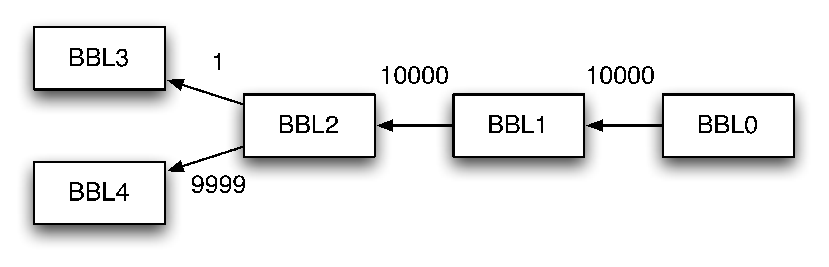
\includegraphics[width=0.64\linewidth]{figs/cfg0.eps}
    \caption{Example control flow graph. Nodes represent basic blocks and edges
    are control transfers. During dynamic profiling, we count how many times
    each edge is followed (edge labels). \label{fig:cfg0}}
\end{figure}

\subsubsection{Memory Integrity Tool (Memcheck)}

Memory integrity tools~\cite{memcheck, drmemory:cgo2011, asan} are designed to
assist developers by reporting (a) memory leakage errors implemented by
instrumenting known memory allocator and deallocator routines to check whether
a program terminates not deallocating any allocated memory chunks and (b) usage
of uninitialized variable by tracking its propagations according to the rules
specified from Table~\ref{tab:memcheck_tracking}. The tool reports the usage of
such uninitialized variables at any point of the program execution.
%
DFT shares much of its architectural characteristics with memory integrity
tools since they utilize shadow memory to track the status of real memory space
while updates are made to the shadow memory by their tracking logic.

Table~\ref{tab:memcheck_tracking} introduces interpretation summary for memory
integrity tool which are different from DFT's interpretation (
Table~\ref{tab:dft_tracking}). One peculiarity that we want examine is that the
checking operation (for the usage uninitialized variables) is far more frequent
in this case, as it is verified before every memory reference.

\begin{table}[h]
        \centering
\begin{tabular}{|l|l|}
\hline
{\bf Instruction} & {\bf Tag propagation rule} \\ \hline \hline
    {\tt \specialcell{ALU-OP OP1 $\leftarrow$ OP2 \\ (add, sub \dots)}} & 
    {\tt t(op1) $\vert=$ t(op2)}\\ \hline
    {\tt MOV OP1  $\leftarrow$  OP2} & {\tt t(op1) = t(op2)}     \\ \hline
    {\tt LOAD OP1 $\leftarrow$ [OP2]} & {\tt t(OP1) = t([OP2])}  \\ \hline
    {\tt STORE [OP1] $\leftarrow$ OP2} & {\tt t([OP1]) = t(OP2)} \\ \hline
\end{tabular}
\caption{presents an interpretation of DFT semantics for pseudo instruction set
architecture.}
\label{tab:memcheck_tracking}
\end{table}

To extend \sreplica to support the tool of this kind, we have to make changes
its components that include (a) binary analyzer that translates {\tt x86}
instructions into intermediate representation (\tfa), (b) analysis component
that perform optimizations against the representation.  Even though changes are
fundamental to its core architecture, we still need to clarify how system
behaviors would change in respond to the modifications we make. 

\subsection{Instrumentation Infrastructure Study}
\label{ssec:inst_infra}

As we have discussed from Section~\ref{ssec:prev_eval}, it is the cost to
instrument the application thread to inline event collector that accounts for
the largest portion of the slowdown. In this section, we discuss about
alternatives for this substrate to improve the overall response time. Firstly,
we compare three different DBI frameworks including PIN DBI our choice for
\sreplica and then move on to cover different approaches based on
software~\cite{brewriting:usenix2003, DTrace} and
hardware~\cite{raksha:isca2007, lba:isca2008} assisted instrumentation. 

\subsubsection{DBI Comparison Study} 
\label{ssec:dbi_study}

Dynamic binary instrumentation (DBI) frameworks enable the development of
program analysis tools for unknown binary by facilitating automated low-level
instrumentation. This technology takes advantage of the process-level
virtualization populating the code cache entries that combines original codes
with users-authored analysis logics. This technique has become essential
building blocks in developing tools that enhance the security and reliability
of software systems.  Representative frameworks of this kind are
PIN~\cite{pin:pldi2005}, Valgrind~\cite{valgrind}, and
DynamoRIO~\cite{dynamorio}.
%
Placed in the same layer between a running application and underlying operating
system, each framework comes with different capabilities and performance
implications as each framework’s design principles varies up to their intended
application domain. However, developers who want to leverage the technology
were rarely informed regarding how to choose a right framework that would serve
best to their purpose.
%
In this work, we compare three aforementioned frameworks by carefully examining
three different aspects – efficiency, capability, and usability. Purpose of our
work is to provide a proper guideline to developers who want to develop
security analysis tools enhancing this technology.

\subsubsection{Other Software Instrumentation Approaches}
\label{ssec:sw_inst}

Trade-off to flexibility of instrumentation leveraging DBI framework based
process-wide virtualization, it cost users to pay high overhead in the course
of translating the binary, interleaving with analysis logic, store those into
the code-cache for future re-use. Having this in mind, we want to explore
feasible alternatives (software approaches but not based on virtualization
technologies) that can replace the layer with less overhead. Ones that we are
actively looking into are solutions based on {\it binary re-writing}~\cite{cfi,
brewriting:usenix2003} and also want to extend light-weighted system
tracing/monitoring frameworks similar to {\it DTrace}~\cite{DTrace} technology.

\subsubsection{Hardware Assisted Instrumentation} 
\label{ssec:hw_inst}

We are also considering to hardware based instrumentation to enhance
\sreplica's execution model. Chen \etal already proposed log based architecture
(LBA)~\cite{lba:isca2008}, a framework for decoupled analysis having hardware
level support, but it's initial prototype failed to address the issue of too
much amount of information collected from the application and transferred using
shared cache connecting two different core which is later resolved by the
software side optimization. 
%
Our insight is that we can use \sreplica's approach to handle excessive amount
of communication volume and frequency to tackle the issue. Furthermore, our
optimal data representation of effective addresses (EAs) and control transfer
trace (BBID), needed to replicate inline monitors, would reduce the size of
required hardware component.
%
The main design and implementation challenges are (a) reduction in space
requirement for additional hardware component and (b) flexible support of
different monitoring logics without requiring hardware logic update.


\begin{figure}[tb]
    \centering
    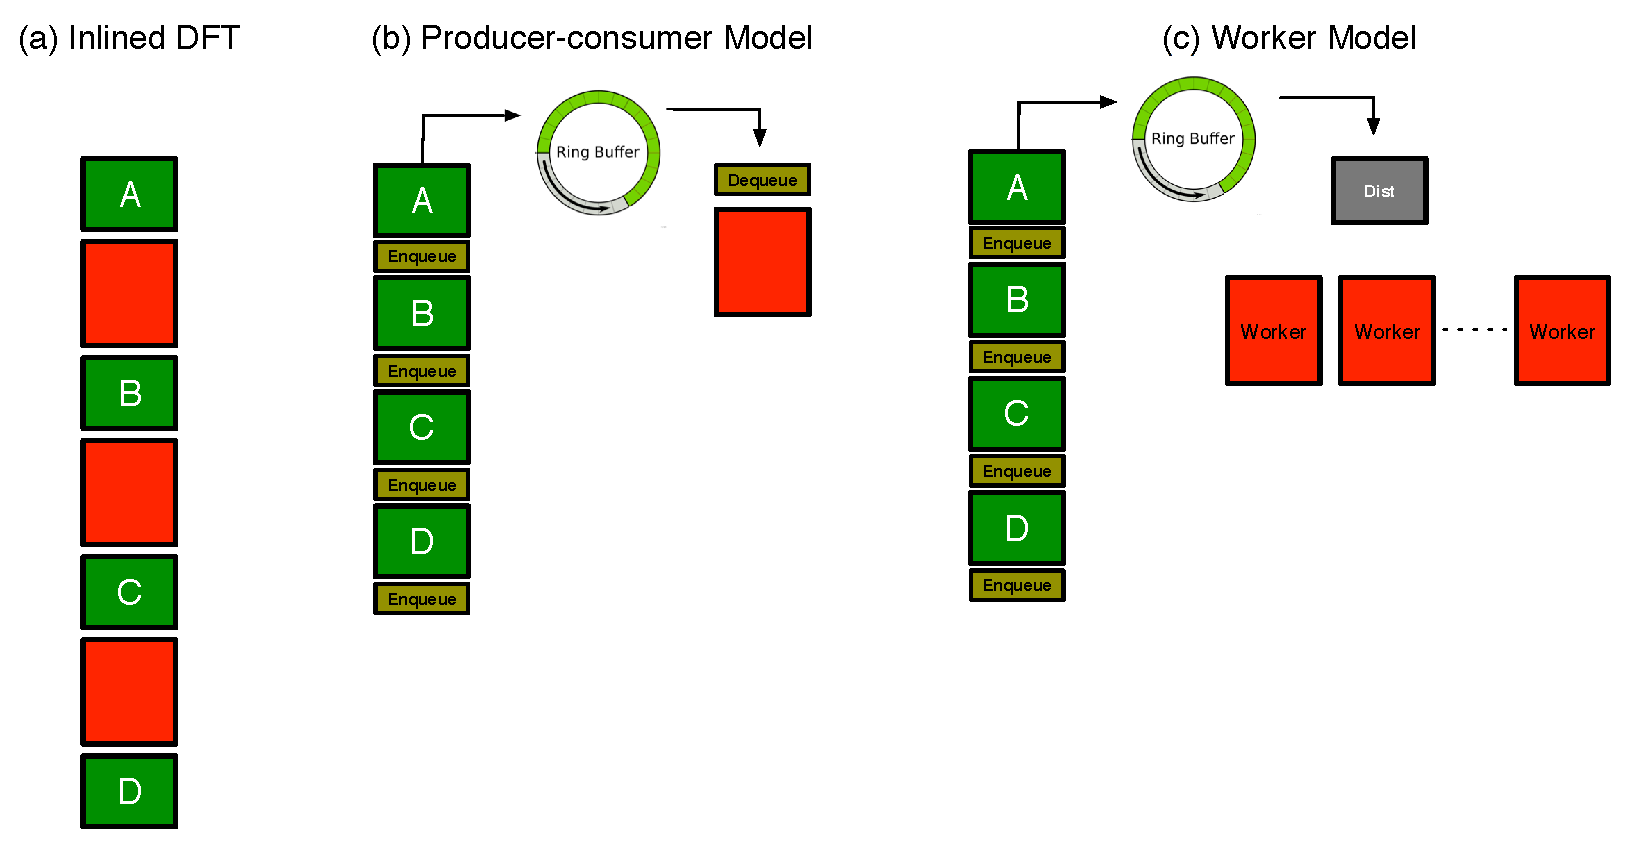
\includegraphics[width=0.90\linewidth]{figs/model0.eps}

    \caption{present three different models to instrument inline monitors. From
    the left to right it has (a) inlining model, (b) a producer - a consumer
    model, and (c) one producer - multiple consumers model.\label{fig:model0}}

\end{figure}

\subsection{Overhead Modeling Framework}

Inline monitors that we discussed from Section~\ref{ssec:inline} may have
different performance implications and become slower being parallelized than
when the monitoring logic is in-lined into a original process. Or we may find
some other execution model what would work better for a monitor. For instance,
when the monitoring logic is too heavy-weighted, it is better to distribute
workloads over multiple number of the worker threads having a arbitrator
thread. Formalizing the idea, we consider three different models presented from
Figure~\ref{fig:model0} to categorize inline monitors.

\begin{itemize}

    \item{{\bf Inlining model:} Inline monitor shows the best response time
            when the monitoring logic is interleaved with the application
    thread. Simple monitors such as call graph profiler falls into this
    category.}

    \item{{\bf $1-1$ model:} Inline monitor shows the best response time when
            an analysis thread is assigned to each application thread. This
    model is same as produce-consumer design pattern. \sreplica implements this
    model parallelizing DFT analysis.}

    \item{{\bf $1-n$ model:} Inline monitor shows the best response time when
            more than one analysis threads are assigned to each application
    thread. This model requires dedicated dispatcher thread for scheduling. To
    be suitable for this model, analysis need to be heavy-weighted and have
    weak data dependency. Cache simulation falls into this category.}

\end{itemize}

%
Given that we have three different execution models, we want to establish an
analytic framework that would take one of in-lined model as an input and
determine the suitable model for the best response time. Once we establish the
framework, we expect to see how performance implications changes from the
modeling framework as we make changes to confirm other hypotheses we discussed
from Section~\ref{ssec:general} and Section~\ref{ssec:inst_infra} 

Ha\etal\cite{cab:oopsala2009} proposed a model simpler than our by taking only
two execution models of {\it Inlining model} (Figure~\ref{fig:model0} (a)), and
{\it $1-1$ model} (Figure~\ref{fig:model0} (b)) into its consideration. By not
having a model for Figure~\ref{fig:model0} (c), their model cannot cover cases
where we have too expensive monitoring logic or the cost for event collector
and its instrumentation become very thin. Furthermore, their purpose of having
the model is different from ours not to choose best model for different
monitors.  In our case, dynamic profiler will be used to capture performance
characteristics of target application and monitors to be analyzed. Based on
profiling result, we expect the framework can better categorize inline monitors 
to have best response time.

As we noted from previous sections, we attempt to change the performance
characteristics by \sreplica and examining instrumentation layer for better
performance. The modeling framework would be a meaningful contribution, if we
can confirm the benefits and disadvantages of these choices ahead of time.
 



